
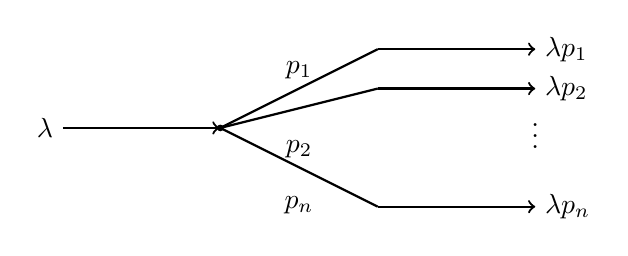
\begin{tikzpicture}
    % Draw the input arrow
    \draw[->, thick] (-2, 0) -- (-0.01, 0);
    \node[left] at (-2, 0) {$\lambda$};

    % Draw the branching point
    \filldraw (0, 0) circle (1pt);

    % Draw the branches
    \draw[thick] (0, 0) -- (2, 1);
    \draw[thick] (0, 0) -- (2, 0.5);
    \draw[thick] (0, 0) -- (2, -1);

    % Labels for probabilities
    \node[above] at (1, 0.5) {$p_1$};
    \node[above] at (1, -0.5) {$p_2$};
    \node[below] at (1, -0.75) {$p_n$};

    % Draw the output arrows for each branch
    \draw[->, thick] (2, 1) -- (4, 1);
    \draw[->, thick] (2, 0.5) -- (4, 0.5);
    \draw[->, thick] (2, -1) -- (4, -1);

    % Labels for the output flows
    \node[right] at (4, 1) {$\lambda p_1$};
    \node[right] at (4, 0.5) {$\lambda p_2$};
    \node at (4, 0) {$\vdots$};
    \node[right] at (4, -1) {$\lambda p_n$};
\end{tikzpicture}
